% Copyright 2014 Imperial College London. All rights reserved.

\documentclass[a4paper,11pt]{report}
\usepackage[top=3cm, bottom=3cm, left=3cm, right=3cm]{geometry}
\usepackage[T1]{fontenc}
\usepackage[utf8]{inputenc}
\usepackage{lmodern}
\usepackage{tikz}

\title{Firedrake-Fluids User Manual}
\author{Imperial College London}

\begin{document}

\maketitle
\tableofcontents

\setlength{\parskip}{0.3cm}
\setlength{\parindent}{0cm}

\chapter{Introduction}
Firedrake-Fluids is a collection of numerical models for the study of fluid dynamics. It uses the Firedrake framework (\texttt{http://firedrakeproject.org/}) to automate the solution of the governing equations written in their weak form using the Unified Form Language.

\chapter{Shallow water}
The shallow water model solves the non-linear version of the shallow water equations. The free surface is split up into a mean component $H$, and a perturbation component $h$ (see Figure \ref{fig:shallow_water_setup}).

\begin{figure}
   \centering
   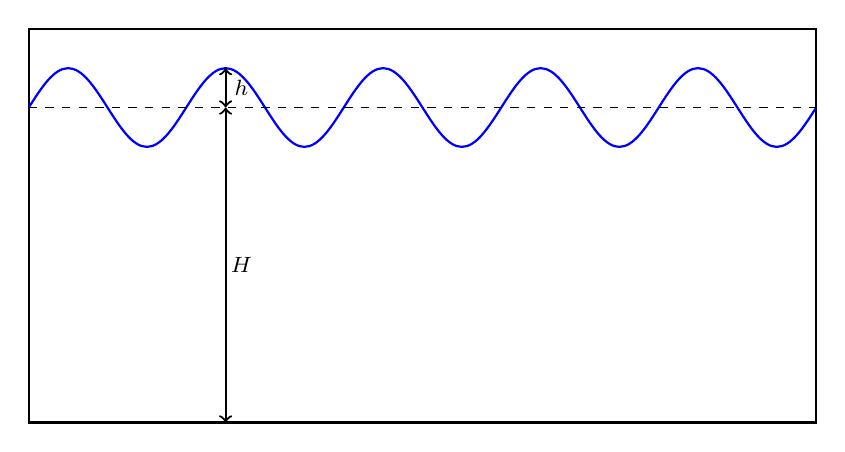
\begin{tikzpicture}
      % Draw the main box     
      \draw[style={thick}] (0, 0) -- (0, 5) -- (10, 5) -- (10, 0) -- cycle;
         
      % Draw the sine curves
      \draw[x=0.5cm,y=1cm, thick, blue] 
        (0,4) sin (1,4.5) cos (2,4) sin (3,3.5) cos (4,4) sin (5,4.5) cos (6,4) sin (7,3.5) cos (8,4)
              sin (9,4.5) cos (10,4) sin (11,3.5) cos (12,4) sin (13,4.5) cos (14,4) sin (15,3.5) cos (16,4) sin (17,4.5) cos (18,4) sin (19,3.5) cos (20,4);

      \draw[style={dashed}] (0, 4) -- (10, 4);

      \draw[arrows=<->, style={thick}] (2.5, 0) -- (2.5, 4);
      \draw (2.7, 2) node{\footnotesize $H$};
      \draw[arrows=<->, style={thick}] (2.5, 4) -- (2.5, 4.5);
      \draw (2.7, 4.25) node{\footnotesize $h$};
      
      \end{tikzpicture}
      \caption{Single-layer shallow water set-up.}
      \label{fig:shallow_water_setup}
   \end{figure}


\section{Model equations}
The shallow water equation set comprises a momentum equation and a continuity equation, each of which are defined below.

\subsection{Momentum equation}
The momentum equation is solved in non-conservative form such that
\begin{equation}
   \frac{\partial \mathbf{u}}{\partial t} + \mathbf{u}\cdot\nabla\mathbf{u} = -g\nabla h + \nabla\cdot\tau - C_D\frac{||\mathbf{u}||\mathbf{u}}{(H + h)},
\end{equation}
where $g$ is the acceleration due to gravity, $\mathbf{u}$ is the velocity, and $C_D$ is the non-dimensional drag coefficient. The stress tensor $\tau$ is given by 
\begin{equation}
   \nu\nabla\mathbf{u},
\end{equation}
where $\nu$ is the kinematic viscosity.

\subsection{Continuity equation}
The continuity equation is given by
\begin{equation}
   \frac{\partial h}{\partial t} + \nabla\cdot\left(\left(H + h\right)\mathbf{u}\right) = 0.
\end{equation}

\section{Configuration}
The model requires three fields to be set up:
\begin{itemize}
   \item Velocity (a prognostic field)
   \item FreeSurfacePerturbation (a prognostic field)
   \item FreeSurfaceMean (a prescribed field)
\end{itemize}

\subsection{Drag}
To include the quadratic drag term in the momentum equation, the drag coefficient field must be enabled and the drag coefficient $C_D$ must be specified.

\subsection{Boundary conditions}
Strong Dirichlet boundary conditions can be enforced for both the FreeSurfacePerturbation and Velocity fields by selecting the \texttt{dirichlet} type. Imposing a no-normal flow condition for velocity can currently only be done weakly by integrating the continuity equation by parts and selecting the \texttt{no\_normal\_flow} boundary condition type in the configuration options.

\section{Current limitations}
\begin{itemize}
   \item Only a continuous Galerkin discretisation may be used (for all fields).
\end{itemize}

\chapter{Stabilisation methods}

\section{Streamline upwind}


\chapter{Diagnostic fields}

\section{Courant number}
The Courant number diagnostic computes the field defined by
\begin{equation}
   \frac{||\mathbf{u}||\Delta t}{\Delta x},
\end{equation}
where $\Delta t$ is the time-step size and $\Delta x$ is the element size (more specifically, it is twice the element's circumradius).

\section{Divergence}
This diagnostic field computes the divergence
\begin{equation}
   \nabla\cdot\mathbf{u},
\end{equation}
of a vector field $\mathbf{u}$.


\end{document}
